\documentclass{beamer}
\usepackage{import}
\subimport{settings/}{settings-pres}
\graphicspath{{images/}}
\usetheme{Warsaw}

\begin{document}

\title{Тема}
\author{Александр Мелихов}
\institute{Волгоградский государственный технический университет}
\date{Волгоград, 2015}

% Создание заглавной страницы.
\frame{\titlepage}
% Автоматическая генерация содержания.
\frame{\frametitle{Содержание}\tableofcontents}

\begin{frame}{Заголовок слайда}
    Содержимое слайда
\end{frame}

\begin{frame}{Заголовок слайда с картинкой}
    \begin{center}
        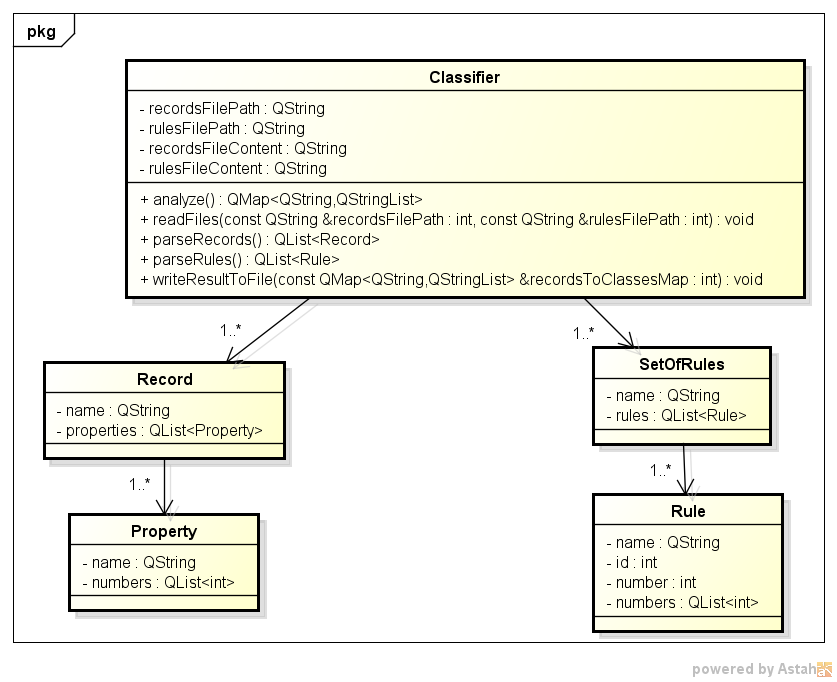
\includegraphics[width=100mm,height=70mm]{class_diagram}
    \end{center}
\end{frame}

\end{document}
